\documentclass[a4paper,11pt]{report}
\usepackage{chuan_math_gkt}
\usetikzlibrary{angles,quotes,intersections,patterns,decorations.pathreplacing}
\chuanexamsetup

\begin{document}
\examfontsize

\examsecret{绝密$\bigstar$启用前}

\examtitle{2020年普通高等学校招生全国统一考试（全国丙卷理科）}{数\quad 学}

\noticetitle
\begin{examnotice}
\item 答卷前，考生务必将自己的姓名、准考证号填写在答题卡上. 
\item 回答选择题时，选出每小题的答案后，用铅笔把答题卡上对应题目的答案标号涂黑. 如需改动，用橡皮擦干净后，再选涂其他答案标号. 回答非选择题时，将答案写在答题卡上. 写在本试卷上无效. 
\item 考试结束后，将本试卷和答题卡一并交回. 
\end{examnotice}

\examsection{一、选择题：本题共12小题，每小题5分，共60分. 在每小题给出的四个选项中，只有一项是符合题目要求的. }
\begin{examquestions}

\item 已知集合 $A=\{(x,y)\mid x,y\in\mathbb N^*,\ y\geq x\}$，$B=\{(x,y)\mid x+y=8\}$，则 $A\cap B$ 中元素的个数为
\fourchoices{$2$}{$3$}{$4$}{$6$}

\item 复数 $\dfrac{1}{1-3\mathrm{i}}$ 的虚部是
\fourchoices{\tallchoice{$-\dfrac{3}{10}$}}{\tallchoice{$-\dfrac{1}{10}$}}{\tallchoice{$\dfrac{1}{10}$}}{\tallchoice{$\dfrac{3}{10}$}}
\item 在一组样本数据中，$1,2,3,4$ 出现的频率分别为 $p_1,p_2,p_3,p_4$，且 $\sum_{i=1}^{4}p_i=1$，则下面四种情形中，对应样本的标准差最大的一组是
\twochoices{$p_1=p_4=0.1$，$p_2=p_3=0.4$}{$p_1=p_4=0.4$，$p_2=p_3=0.1$}{$p_1=p_4=0.2$，$p_2=p_3=0.3$}{$p_1=p_4=0.3$，$p_2=p_3=0.2$}

\item Logistic 模型是常用数学模型之一，可应用于流行病学领域，有学者根据公布数据建立了某地区新冠肺炎累计确诊病例数 $I(t)$（$t$ 的单位：天）的 Logistic 模型：$I(t)=\dfrac{K}{1+e^{-0.23(t-53)}}$，其中 $K$ 为最大确诊病例数. 当 $I(t^*)=0.95K$ 时，标志着已初步遏制疫情，则 $t^*$ 约为（$\ln19\approx3$）
\fourchoices{$60$}{$63$}{$66$}{$69$}
\newpage
\item 设 $O$ 为坐标原点，直线 $x=2$ 与抛物线 $C:y^2=2px(p>0)$ 交于 $D,E$ 两点，若 $OD\perp OE$，则 $C$ 的焦点坐标为
\fourchoices{\tallchoice{$\left(\dfrac14,0\right)$}}{\tallchoice{$\left(\dfrac12,0\right)$}}{$(1,0)$}{$(2,0)$}

\item 已知向量 $\vec a,\vec b$ 满足 $|\vec a|=5$，$|\vec b|=6$，$\vec a\cdot\vec b=-6$，则 $\cos\langle \vec a,\vec a+\vec b\rangle=$
\fourchoices{\tallchoice{$-\dfrac{31}{35}$}}{\tallchoice{$-\dfrac{19}{35}$}}{\tallchoice{$\dfrac{17}{35}$}}{\tallchoice{$\dfrac{19}{35}$}}

\item 在 $\triangle ABC$ 中，$\cos C=\dfrac23$，$AC=4$，$BC=3$，则 $\cos B=$
\fourchoices{\tallchoice{$\dfrac19$}}{\tallchoice{$\dfrac13$}}{\tallchoice{$\dfrac12$}}{\tallchoice{$\dfrac23$}}

\item 右图为某几何体的三视图，则该几何体的表面积是

\begin{tightcenter}
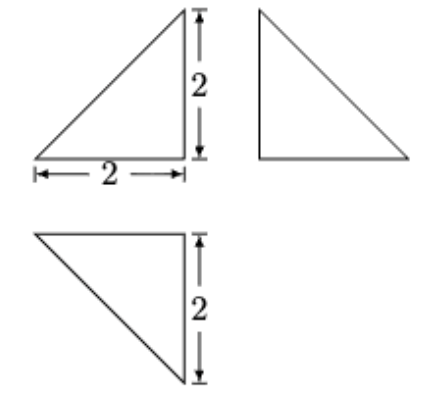
\includegraphics[width=3cm]{figures/2020_xkb3_li_image19.png}
\end{tightcenter}

\fourchoices{$6+4\sqrt2$}{$4+4\sqrt2$}{$6+2\sqrt3$}{$4+2\sqrt3$}

\item 已知 $2\tan\theta-\tan\left(\theta+\dfrac{\pi}{4}\right)=7$，则 $\tan\theta=$
\fourchoices{$-2$}{$-1$}{$1$}{$2$}

\item 若直线 $l$ 与曲线 $y=\sqrt{x}$ 和圆 $x^2+y^2=\dfrac15$ 都相切，则 $l$ 的方程为
\fourchoices
{$y=2x+1$}
{\tallchoice{$y=2x+\dfrac12$}}
{\tallchoice{$y=\dfrac12x+1$}}
{\tallchoice{$y=\dfrac12x+\dfrac12$}}

\item 设双曲线 $C:\dfrac{x^2}{a^2}-\dfrac{y^2}{b^2}=1(a>0,b>0)$ 的左、右焦点分别为 $F_1,F_2$，离心率为 $\sqrt5$. $P$ 是 $C$ 上一点，且 $F_1P\perp F_2P$. 若 $\triangle PF_1F_2$ 的面积为 $4$，则 $a=$
\fourchoices{$1$}{$2$}{$4$}{$8$}

\item 已知 $5^5<8^4$，$13^4<8^5$. 设 $a=\log_5 3$，$b=\log_8 5$，$c=\log_{13}8$，则
\fourchoices{$a<b<c$}{$b<a<c$}{$b<c<a$}{$c<a<b$}

\end{examquestions}

\examsection{二、填空题：本题共4小题，每小题5分，共20分. }
\begin{examquestions}[start=13]

\item 若 $x,y$ 满足约束条件\linsys{x+y\geq0\\2x-y\geq0\\x\leq1}，则 $z=3x+2y$ 的最大值为 \blank.

\item $\left(x^2+\dfrac2x\right)^6$ 的展开式中常数项是 \blank.（用数字作答）

\item 已知圆锥的底面半径为 $1$，母线长为 $3$，则该圆锥内半径最大的球的体积为 \blank.

\item 关于函数 $f(x)=\sin x+\dfrac{1}{\sin x}$ 有如下四个命题：

\gktcircled{1} $f(x)$ 的图像关于 $y$ 轴对称. \gktcircled{2} $f(x)$ 的图像关于原点对称. 

\gktcircled{3} $f(x)$ 的图像关于直线 $x=\dfrac{\pi}{2}$ 对称. \gktcircled{4} $f(x)$ 的最小值为 $2$. 

其中所有真命题的序号是 \blank.

\end{examquestions}

\examsection{三、解答题：共70分. 解答应写出文字说明、证明过程或演算步骤. 第17题～第21题为必考题，每个试题考生都必须作答. 第22、23题为选考题，考生根据要求作答. }
\begin{examanswers}[start=17]

\item（12分）

设数列 $\{a_n\}$ 满足 $a_1=3$，$a_{n+1}=3a_n-4n$. 

\subq{（1）}{计算 $a_2,a_3$，猜想 $\{a_n\}$ 的通项公式并加以证明；}

\subq{（2）}{求数列 $\{2^n a_n\}$ 的前 $n$ 项和 $S_n$. }
\vspace{-1em}
\item（12分）

某学生兴趣小组随机调查了某市 $100$ 天中每天的空气质量等级和当天到某公园锻炼的人次，整理数据得到下表（单位：天）：

\begin{tightcenter}
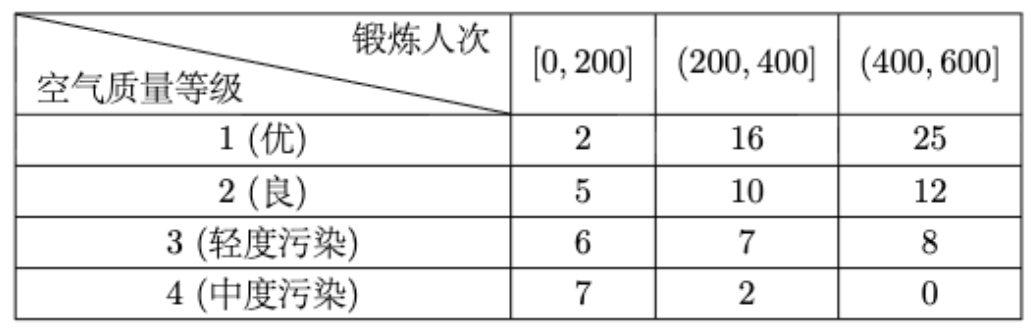
\includegraphics[width=9cm]{figures/2020_xkb3_li_image31.png}
\end{tightcenter}

\subq{（1）}{分别估计该市一天的空气质量等级为 $1,2,3,4$ 的概率；}

\subq{（2）}{求一天中到该公园锻炼的平均人次的估计值（同一组中的数据用该组区间的中点值为代表）；}

\subq{（3）}{若某天的空气质量等级为 $1$ 或 $2$，则称这天“空气质量好”；若某天的空气质量等级为 $3$ 或 $4$，则称这天“空气质量不好”. 根据所给数据，完成下面的 $2\times2$ 列联表，并根据列联表，判断是否有 $95\%$ 的把握认为一天中到该公园锻炼的人次与该市当天的空气质量有关？}

\begin{tightcenter}
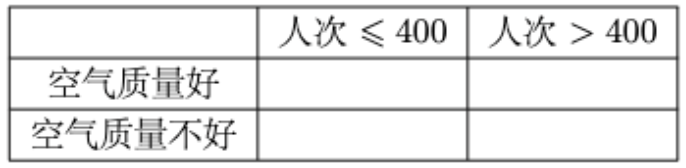
\includegraphics[width=6cm]{figures/2020_xkb3_li_image32.png}
\end{tightcenter}

附：$K^2=\dfrac{n(ad-bc)^2}{(a+b)(c+d)(a+c)(b+d)}$. 

\begin{tightcenter}
{\renewcommand{\arraystretch}{0.9}
\begin{tabular}{|c|c|c|c|}
\hline
$P(K^2\geq k)$ & $0.050$ & $0.010$ & $0.001$\\
\hline
$k$ & $3.841$ & $6.635$ & $10.828$\\
\hline
\end{tabular}}
\end{tightcenter}

\item（12分）

如图，在长方体 $ABCD-A_1B_1C_1D_1$ 中，点 $E,F$ 分别在棱 $DD_1,BB_1$ 上，且 $2DE=ED_1$，$BF=2FB_1$. 

\noindent\begin{minipage}[t]{0.66\linewidth}
\subq{（1）}{证明：点 $C_1$ 在平面 $AEF$ 内；}

\subq{（2）}{若 $AB=2$，$AD=1$，$AA_1=3$，求二面角 $A-EF-A_1$ 的正弦值. }
\end{minipage}\hfill
\begin{minipage}[t]{0.17\linewidth}
\vspace{-1.9em}
\centering
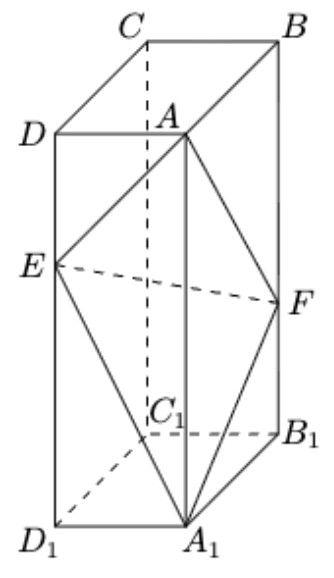
\includegraphics[width=\linewidth]{figures/2020_xkb3_li_image35.png}
\end{minipage}
\vspace{-3em}

\item（12分）

已知椭圆 $C:\dfrac{x^2}{25}+\dfrac{y^2}{m^2}=1(0<m<5)$ 的离心率为 $\dfrac{\sqrt{15}}{4}$，$A,B$ 分别为 $C$ 的左、右顶点. 

\subq{（1）}{求 $C$ 的方程；}

\subq{（2）}{若点 $P$ 在 $C$ 上，点 $Q$ 在直线 $x=6$ 上，且 $|BP|=|BQ|$，$BP\perp BQ$，求 $\triangle APQ$ 的面积. }

\item（12分）

设函数 $f(x)=x^3+bx+c$，曲线 $y=f(x)$ 在点 $\left(\dfrac12,f\left(\dfrac12\right)\right)$ 处的切线与 $y$ 轴垂直. 

\subq{（1）}{求 $b$；}

\subq{（2）}{若 $f(x)$ 有一个绝对值不大于 $1$ 的零点，证明：$f(x)$ 所有零点的绝对值都不大于 $1$. }

\item（10分）【选修4-4：坐标系与参数方程】

在直角坐标系 $xOy$ 中，曲线 $C$ 的参数方程为\linsys{x=2-t-t^2\\y=2-3t+t^2}（$t$ 为参数且 $t\ne1$），$C$ 与坐标轴交于 $A,B$ 两点. 

\subq{（1）}{求 $|AB|$；}

\subq{（2）}{以坐标原点为极点，$x$ 轴正半轴为极轴建立极坐标系，求直线 $AB$ 的极坐标方程. }

\item（10分）【选修4-5：不等式选讲】

设 $a,b,c\in\mathbb R$，$a+b+c=0$，$abc=1$. 

\subq{（1）}{证明：$ab+bc+ca<0$；}

\subq{（2）}{用 $\max\{a,b,c\}$ 表示 $a,b,c$ 的最大值，证明：$\max\{a,b,c\}\geq\sqrt[4]{3}$. }

\end{examanswers}

\end{document}